\documentclass[11pt]{article}
\usepackage[margin=1in]{geometry}
\usepackage{amsmath,amssymb}
\usepackage{graphicx}
\usepackage[hidelinks]{hyperref}

\title{Literature Status: Summable Szlenk Index and Injective Tensor Products}
\author{FA/Banach run \texttt{fa\_banach\_001}}
\date{2026-06-13}

\begin{document}
\maketitle

\section*{Status}

This is a literature-already-answered packet, not an original proof from the
run.  Draga--Kochanek, arXiv:1604.03461, ask whether
\[
  X\widehat{\otimes}_{\varepsilon}Y
\]
has summable Szlenk index whenever $X$ and $Y$ are separable Banach spaces
with summable Szlenk index.  Causey, arXiv:1707.08170, answers this
affirmatively, and in a stronger form.

\section*{Original Question}

The original source is:

\begin{quote}
S. Draga and T. Kochanek, \emph{The Szlenk power type and tensor products of
Banach spaces}, arXiv:1604.03461.
\end{quote}

At the end of the paper, after proving results on Szlenk power type and
separable determination, the authors ask whether the injective tensor product
of two separable Banach spaces with summable Szlenk index must again have
summable Szlenk index.

\begin{center}
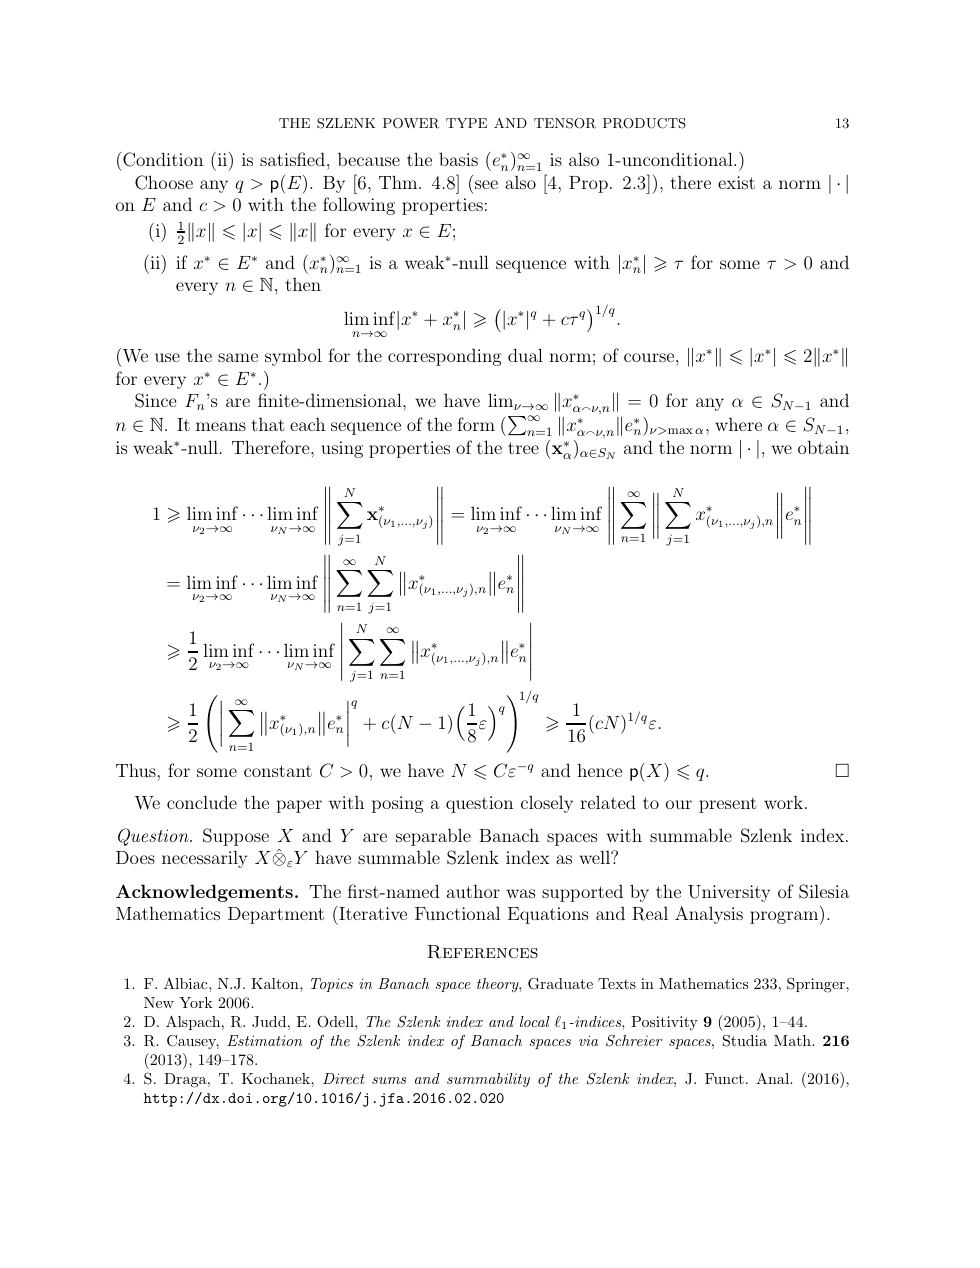
\includegraphics[width=\textwidth]{figures/dk_question_page13.png}
\end{center}

\section*{Later Answer}

The supporting source is:

\begin{quote}
R. M. Causey, \emph{Concerning summable Szlenk index}, arXiv:1707.08170.
\end{quote}

Causey's abstract states that the paper proves that the injective tensor
product of two Banach spaces has summable Szlenk index if both spaces do, and
that this answers a question from Draga--Kochanek.  The operator-level
statement is Theorem 1.3: if $A_0$ and $A_1$ have summable Szlenk index, then
so does
\[
  A_0\otimes A_1:
  X_0\widehat{\otimes}_{\varepsilon}X_1
  \longrightarrow
  Y_0\widehat{\otimes}_{\varepsilon}Y_1,
\]
with the converse when neither operator is zero.

\begin{center}
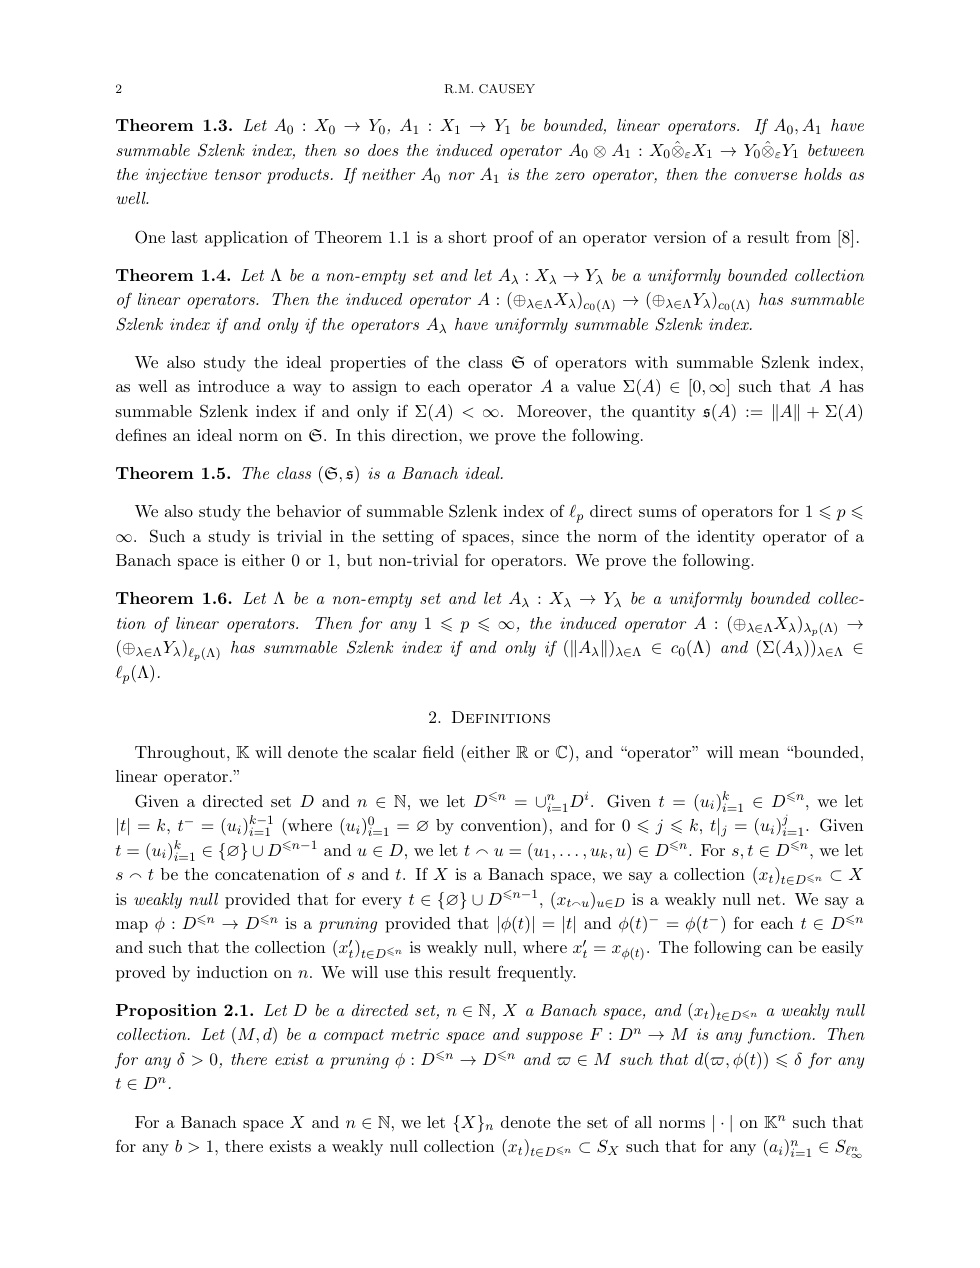
\includegraphics[width=\textwidth]{figures/causey_theorem_page2.png}
\end{center}

The space-level answer is Corollary 5.3:
\[
  X_0\widehat{\otimes}_{\varepsilon}X_1
  \text{ has summable Szlenk index}
  \quad\Longleftrightarrow\quad
  X_0 \text{ and } X_1 \text{ do},
\]
for non-zero Banach spaces $X_0,X_1$.  The same corollary gives the equivalent
asymptotic $c_0$ formulation.

\begin{center}
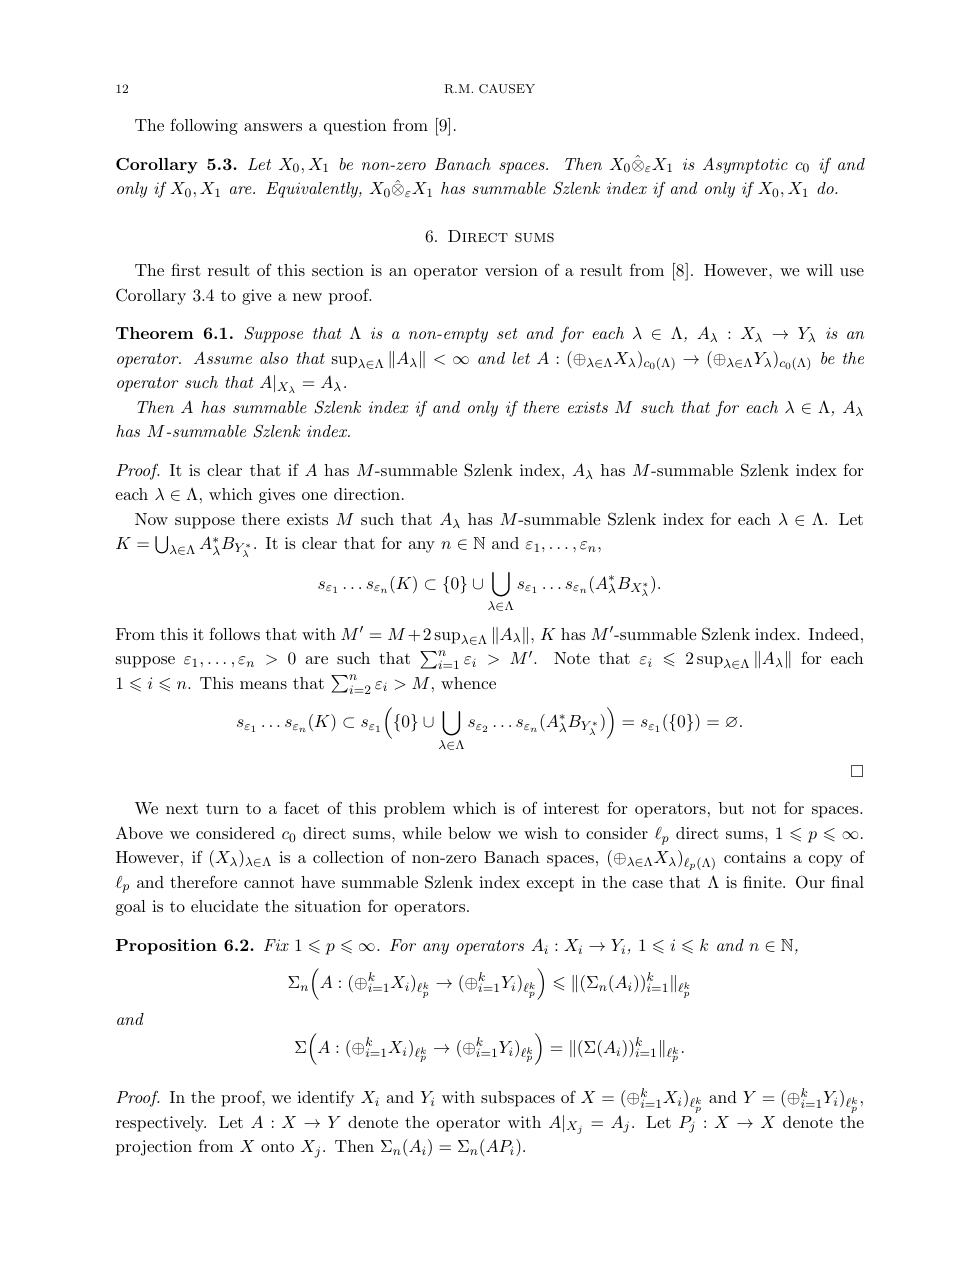
\includegraphics[width=\textwidth]{figures/causey_corollary_page12.png}
\end{center}

\section*{Verification Notes}

This is a separate-source answer.  The original paper poses the question at
the end; Causey's later paper cites the Draga--Kochanek paper as reference
[9] and explicitly says that the tensor-product result answers a question
from that reference.  Causey's Corollary 5.3 is stronger than the original
question because it removes separability and proves an if-and-only-if
statement for non-zero spaces.

\section*{Search Bounds}

The run registry, solution README, and active-claim directory were checked for
overlapping entries involving arXiv:1604.03461, arXiv:1707.08170, Draga,
Kochanek, Causey, summable Szlenk index, and injective tensor products.  The
original and supporting arXiv PDFs were downloaded and inspected locally.  No
MathSciNet or Zentralblatt search was performed.

\section*{Review Recommendation}

Verify the final question in arXiv:1604.03461 and Corollary 5.3 in
arXiv:1707.08170.  The status transfer relies only on this explicit question
and Causey's explicit later answer.

\end{document}
